\section{Implementación}

Respecto a la implementación, el software para balancear las clases está implementado en Python mientras que los algoritmos utilizados están implementados en C++.

\subsection{Preprocesado}

De cara al preprocesado simplemente se han implementado funciones que reciben como entrada los datos y realizan las correspondientes transformaciones, así como funciones para realizar un conteo de clases. También se ha desarrollado un script en Python que será el encargado de realizar el sobremuestreo de datos para las clases minoritarias, como se comento en la sección del preprocesado de datos.

\subsection{Algoritmos}

Con respecto a la implementación de los algoritmos utilizados, estos se han implementado en C++.

\begin{figure}[H]
	 \centering
	 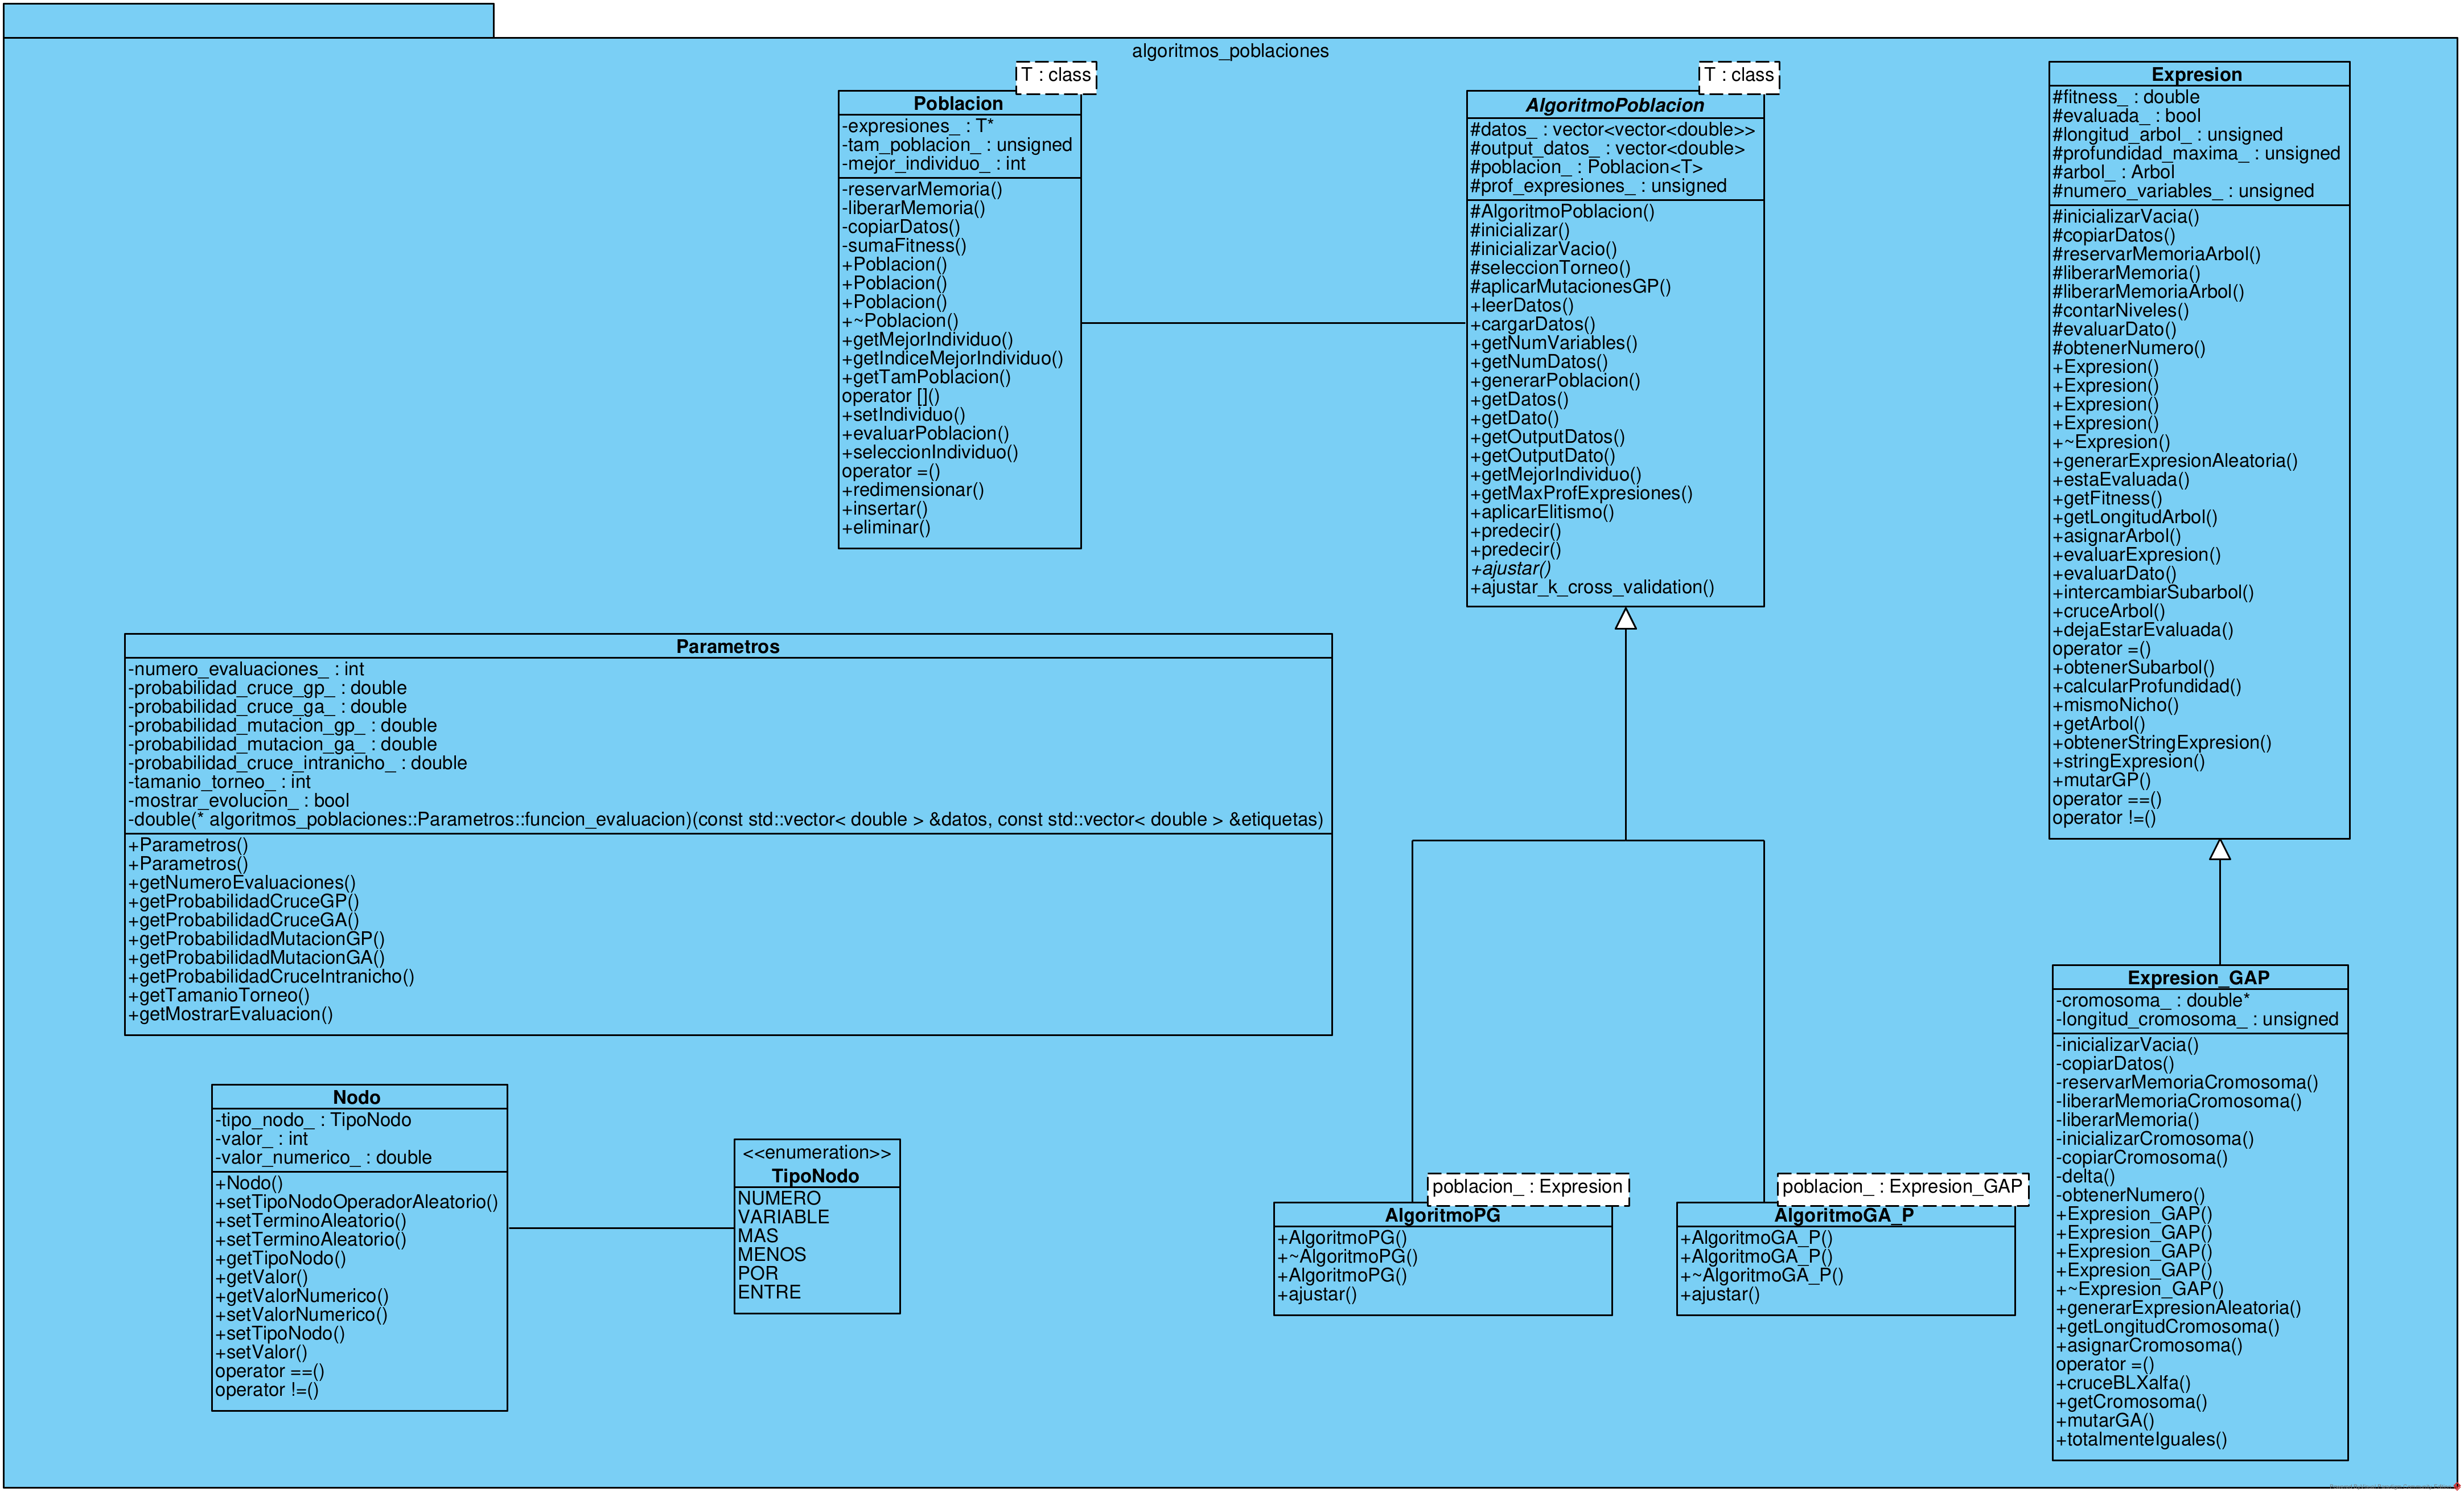
\includegraphics[width=\textwidth]{diagrama_clases.png}
	 \caption{Diagrama de clases.}
	\label{fig:diagrama_clases}
\end{figure}
